\documentclass[thesis.tex]{subfiles}
\begin{document}
\chapter{Introduction}

%\todo{%
%  This chapter should introduce:
%  \begin{itemize}
%  \item Introduce the thesis.
%  \item State the main contributions.
%  \end{itemize}
%
%  We should also ask \emph{what is the thesis of the thesis} which is a fiddly
%  way of asking what are we trying to prove with this document?
%}

\begin{figure}
  \centering
  \includegraphics[width=\linewidth]{figures/mobile-ecosystem.png}
  \caption{Interactions surrounding the use of mobile devices.}
  \label{fig:mobile-ecosystem}
\end{figure}

Mobile devices are ubiquitous, yet the relationships between their users, and
the environment they run in is often vague. Users have preferences for the apps
they use. Stores have terms for the apps they sell, and for the users who buy
them. Companies have policies as to what apps and devices employees can use in
the office. The precise trust relationships, however, are often hidden in
informal, or natural language, descriptions of the policies.

As the devices have become more powerful there has been an increasing wish to
control the devices. Companies expect devices to follow their corporate policies
within their networks and trust users to abide by their policies as well as use
tools to enforce some aspects of them. Some users may have reservations about
what data an app can get access to and may wish to restrict the app's access.
Users may rely on stores to vet the apps they sell, but will likely not know (or
necessarily care) precisely how the store checked the app.

These devices exist within the \emph{mobile ecosystem}: which we define as
\textbf{the interactions surrounding the use of smart phones and tablet
computers in a given setting}. Figure~\ref{fig:mobile-ecosystem} shows some of the relationships
between devices, their users and their preferences, the stores, companies and
all these principal's policies. Users have phones or other mobile devices. They
may own personal devices or have a company one. They may have their own
preferred ways of using the device, or they have to follow policies written
by their employer. They download apps, written by developers from app stores,
all with their own policies and some of the stores may delegate some aspects of
their quality control to external vetting software.

Prior work focused on how systems and tools can check and enforce more
sophisticated policies and ever finer controls. This thesis asks a different
question: \textbf{how can we capture the informal policies and trust
relationships surrounding the mobile ecosystem and use formal languages to model
and examine them?} We ask how can we tie the top-level goals in the natural
language policies and preferences to the tools used to implement them? How can
we compare different policies and highlight similarities and differences between
them precisely?

\section{The Need For Policies}

As mobile devices are increasingly capable and hold ever-increasing amounts of
information, users and businesses need to manage how the devices behave.
Employees now bring their mobile devices to work and use them to access company
email and documents. In response to this companies might \emph{mandate} that
employees follow mobile device policies that describe how the employees should
use their devices within the company. These policies vary in terms of formality
inside and outside of a company. 
They may also use \ac{MDM} software, tools which allow companies to configure
mobile devices remotely, to enforce the policies. Regulation, such as
\ac{HIPAA}, may also affect some companies.

A user may never write their personal privacy preferences in a formal language
but they may make decisions guided by them. An example might be a user choosing
which apps to install and which to avoid, based on their own \emph{discretion}.
They may make decisions based on what their friends have told them, or what a
review said about the app.

In this section we will start to introduce by example AppPAL: an authorization
language for the policies of the mobile ecosystem, based on
SecPAL~\cite{becker_secpal:_2006}. We will describe AppPAL in greater detail in
\autoref{chap:apppal} and throughout the thesis. We have implemented SecPAL to
explore its use and build our own policy language called AppPAL to capture the
policies of the mobile ecosystem. Moreover, when we show an AppPAL snippet in
\framebox{\texttt{teletype font}} it can be parsed and used as part of a
policy\footnote{Sometimes with minimal edits as some constraints used are not
implemented.} with our \emph{AppPAL} interpreter (described in
\autoref{chap:apppal}).


A key aspect of the mobile ecosystem is \emph{delegation}. The user of a mobile
device (typically) first logs on to a Google or Apple account before using the
device, which fetches all their data from wherever server stores it. Rather than
keep account information locally an app may prompt the user to log in,
delegating to a third-party (such as Google or Facebook) to manage the account
ID. Capturing these trust relationships as policies can help clarify the precise
terms for authentication and who each principal trusts to make what decisions.
For example, an app might trust Google to manage accounts. Google will only
authorize a user if the user has authorized the app, and will only allow the app
access to the data the user has explicitly authorized:

%\noindent\begin{minipage}{\linewidth}%\vspace{\baselineskip}
\begin{lstlisting}
'app' says 'google' can-say 
  'app' canLink(User:U, Account:A).

'google' says App:A canLink(User:U, Account:Acc)
  if U hasAuthorized(A), U hasAccount(Acc).

'google' says User:U can-say U hasAuthorized(App:A)
  if U isAuthenticatedWith(Token), Token isValid.

'google' says User:U can-say App:A canAccess(Data:D)
  if D isOwnedBy(U).
\end{lstlisting}
%\end{minipage}

Users may install apps manually themselves, but they might also buy and download
apps from one or more app stores. They trust these app stores to sell them
\emph{good and safe} apps, and delegate the checking of them to the store.
Whereas, in the earlier days of PCs, a user might once have done the check
themselves (or at least delegated to an \ac{AV} package on their computer) now
the responsibility is with the stores. Now most apps come signed either by the
developer who created it (in the case of Google's Play Store), the store that
sold it (in the case of Amazon's app store) or both (Apple's App Store). These
signatures ensure integrity and some measure of authenticity, standing for an
assertion that the signer makes that the app is safe to run. For example we may
take Apple's signature as an assertion that Apple's vetting process has approved
the app is safe to use by its customers. A store may delegate to a third-party
app vetting service to assess what apps are safe (Yandex and Aptoide stores), or
use their own in-house teams.

Users sometimes recommend apps to each other. We can capture, for example, that
Alice may trust Bob to tell her which apps are good.
%
\begin{lstlisting}
'alice' says 'bob' can-say App:A isGood.
\end{lstlisting}
%
Some may consider what apps they want to use on their phone and come up with
informally applied personal policies that describe how they want to use them.
They may never write these policies down, but they might take the form of
preferences that influence the apps they choose, by capturing these we can start
to examine and compare policies as well as potentially enforcing them. Bob might recommend any app by Nintendo:
%
\begin{lstlisting}
'bob' says App:A isGood
  if A isGame,
     A hasDeveloper('nintendo').
\end{lstlisting}
%
Bob might trust reviews and review sites to give him an idea of an app's quality. 
%
\begin{lstlisting}
'bob' says App:A isGood
  if A hasReviewScore(N)
  where N > 60.
 
'bob' says 'metacritic' can-say
  App:A hasReviewScore(Percent:N).
\end{lstlisting}
%
Bob might also recommend an app based on its app store categorization and its permissions.
%
\begin{lstlisting}
'bob' says App:A isGood
  if A hasCategory('flashlight'),
     A hasPermissions(P)
  where ! contains(P, 'INTERNET').
\end{lstlisting}

They allow their employers to say how they should their devices, who
may in turn delegate to IT departments, to write rules, which may
delegate back to the users to state what rules they're willing to
follow.

A company looking to control their employee's mobile devices at work might write
a \ac{BYOD} policy. They might also use \ac{MDM} software to control some
aspects of their devices. The company might write these with varying degrees of
formality but often they use natural language. This adds vagueness
and can lead to confusion about how the company upholds the policy. By
describing the policy in a formal language we can express the policy
rigorously. We can start to make comparisons between users, and with rules
for checking the policy start to help the user to make decisions more
accurately, or measure the extent a user follows their stated policy. Using
formal languages we can model the policies precisely, helping clarify their
meanings and make precise comparisons between different policies. We could tie the
rules in the \ac{BYOD} policies to the \ac{MDM} tools used to
check them.

If a company needs to use apps which conform with a policy such as
\ac{HIPAA} they could use static analysis tools to check for some
aspects of the policy.  A company might use
Mallodroid~\cite{fahl_why_2012} to detect when apps send data unencrypted.  
%
\begin{lstlisting}
'company' says Employee:E canUse(App:A)
  if A isHIPAAConformant
  where
    mallodroidCheckSafe(A) = True;
\end{lstlisting}
%
It is important not to confuse the tools and
techniques we might use to uphold parts of a policy with the end
goal of ensuring compliance.  A formal language that
lets us sever the policy from its implementation can help us
understand the policy precisely, and then show precisely how we check the
policy.  It lets us see which tools are checking what rules, and identify gaps where the policy is not
being checked sufficiently.

These trust relationships and delegations permeate the entire mobile
ecosystem.  They represent an important aspect of the ecosystem that a
policy language should catch to describe the
relationships and policies within it.

% \section{History of Mobile Devices}
% 
% \begin{figure}\sffamily\scriptsize
%   \centering
%   \begin{chronology}[5]{1993}{2017}{\textwidth}
%     \event{1993}{Apple Newton}
%     \event{1994}{IBM Simon}
%     \event{1996}{Palm Pilot}
%     \event{1998}{Symbian}
%     \event{1999}{BlackBerry}
%     \event{2000}{\stackanchor{Java Micro Edition and Windows Mobile}{First mobile virus (Timofonica) discovered}}
%     \event{2003}{Nokia N-Gage}
%     \event{2005}{iOS released, Commwarrior-A worm discovered}
%     \event{2008}{Android, iPhone and App Store}
%     \event{2010}{\stackanchor{Windows Mobile becomes Windows Phone}{iPad}}
%     \event{2012}{Symbian discontinued}
%     \event{2013}{Sailfish OS}
%     \event{2015}{\stackanchor{Windows Phone discontinued}{non-Android BlackBerry devices discontinued}}
%   \end{chronology}
%   \caption{Timeline of mobile device developments.}
%   \label{fig:timeline-mobile}
% \end{figure}
% 
% Some of the earliest mobile devices were the \acp{PDA} devices such as Apple's
% Newton and the Palm Pilot. They were portable miniature computers designed to
% store personal information, calendars and notes.  In the 1990s mobile phones were just portable
% telephones, but with the IBM Simon in 1994 these devices started to have the features of a \ac{PDA}, becoming what would later be called a
% \emph{smart phone}. These early smart phones had a telephone connection, unlike
% the \acp{PDA}. The earliest smart phones could use email and fax, as well as
% managing personal information. They were somewhat underpowered compared to the
% \ac{PDA} devices, however.
% 
% In 1998 Symbian released their OS. Symbian devices could install apps, written
% in C++ or Java (if the phone supported JME). They had cameras, could play music.
% They even had early malware which would illicitly send texts to premium rate
% numbers. They were the forebears of the \emph{modern} smart phone. They were
% also starting to become affordable, with the lowest end models starting to be
% affordable. Advertisers marketed devices, like Nokia's N-Gage which had games users could buy for their devices, to
% teenagers. Others, such as
% the BlackBerry, were for business users.
% 
% By the mid-2000s the devices were ubiquitous. In 1999 Microsoft released Windows Mobile. Apple released the first version of iOS the same year. 
% The first modern app store was for iOS in
% 2008\footnote{Earlier attempts resembled Linux package managers.}.
% With increasing amounts of personal information available on these devices
% malware authors started to take note. The first mobile virus was found in 2000
% which sent text messages\footnote{The Timofonica virus infected Windows PCs to
% send text messages via a web based SMS gateway. It was not harmful, only
% irritating.}. By 2005 researchers found the self-replicating Commwarrior worm that ran entirely on smartphones.
% 
% Despite increasing amount of malware, in a blog post from 2006 for Symantec,
% Chien noted that adware and privacy invading apps might become a bigger
% threat~\cite{eric_chien_spyware_2006}. These would likely need new controls to
% help manage user's privacy preferences, an idea that would be picked up by the
% fine-grained permissions research (see \autoref{sec:fine-grained-permissions}).
% 
% \begin{quote}
%   ``While threats exist and are actively spreading, we are probably
%   still years away from the situation we have with the Microsoft Windows
%   [$\cdots$] We have already seen spyware applications for mobile devices
%   (e.g. Spyware.Flexispy) that can monitor activities on the mobile
%   device and then send them to a remote server. [$\cdots$] Just as
%   worrying is the fact that the adware market is just beginning to take
%   notice of mobile devices. Already some Bluetooth advertising schemes
%   have been tested, where a bus stop is outfitted with a device that
%   just spams out messages via Bluetooth.
% 
%   [$\cdots$]
%   
%   So, while worms and Trojans already exist for the mobile
%   platforms, spyware and adware applications are just now gaining a
%   foothold in the mobile device space. Spyware and adware pose a
%   potentially large security issue in the near future, as the companies
%   that produce such applications are less affected by the natural
%   limiting factors.''
% \end{quote}
% 
% \subsection{Modern Mobile Devices}
% 
% In 2008 Apple released the first iPhone, and shortly after Google
% released the Android OS.  Symbian released its last version in
% 2012.  Android had replaced it as the dominant OS on most devices.  
% 
% Android and iOS differ from past efforts, and conventional desktop OSs, as they
% made it far harder to run arbitrary programs. Apple's devices cannot
% run code that Apple has not signed or install software from outside of its App
% Store, which Apple control. Android devices offer a similar app marketplace,
% but where there is less checking of each
% app~\cite{oberheide_dissecting_2012}. Whilst Android users can install software
% from other sources, the option is hidden by default. As well as restrictions to
% software, the OSs are also better hardened. Devices no longer have an all-powerful
% \emph{root} account, and APIs provide controlled access to
% sensitive data to restrict malicious behaviors; such as stopping SMSs being
% sent programatically to premium rate accounts.
% 
% Mobile devices store an increasing amount of personal data about their users.
% They contain address books, records of phone calls, and GPS logs of where their
% users had been. With iOS and Android users have become more aware about privacy
% issues with their devices, in part because of increased media coverage of
% privacy issues.
% 
% A survey by Chin~et~al{.} found that users were more concerned about
% privacy on their mobile devices than on their
% laptops~\cite{chin_measuring_2012}. They found that users of a smart phone were
% more likely to install an app that came recommended from a friend, was popular
% or was free. To subsidize the cost of producing free apps, and to better
% understand how users used their apps, some developers have added adware and
% tracking libraries to their apps. These libraries add
% crash and error tracking, as well as collecting personal data. The developers can sell this data to
% advertisers to subsidize the app's price~\cite{seungyeop_han_study_2012}.
% 
% Many researchers have proposed finer privacy controls, to help users who are increasingly concerned about their
% privacy and apps which are increasingly privacy invading~\cite{jeon_dr._2012,beresford_mockdroid:_2011,conti_crepe:_2010,backes_appguard_2013}.  
% In general, however, users seem confused about how permissions work~\cite{felt_android_2012}. 
% 
% Android and iOS have permissions where users are asked by their
% devices if an app can use certain data when it first requests access to it.
% Users can revoke that decision later if they wish.
% Android's switched to an current \emph{ask on use} permissions model in 2015. 
% Many older Android devices which cannot control permissions are
% still in use. In June 2016 only 10\% of devices used the latest version of
% Android, with around 5\% using a version more than five years old. In contrast 79\% of iOS devices use the latest
% OS, 16\% use the one before and only 5\% use anything
% older~\cite{apple_app_2017}. This means that many Android user's cannot benefit
% from improved privacy controls.
% 
% %\begin{figure}
% %\centering
% %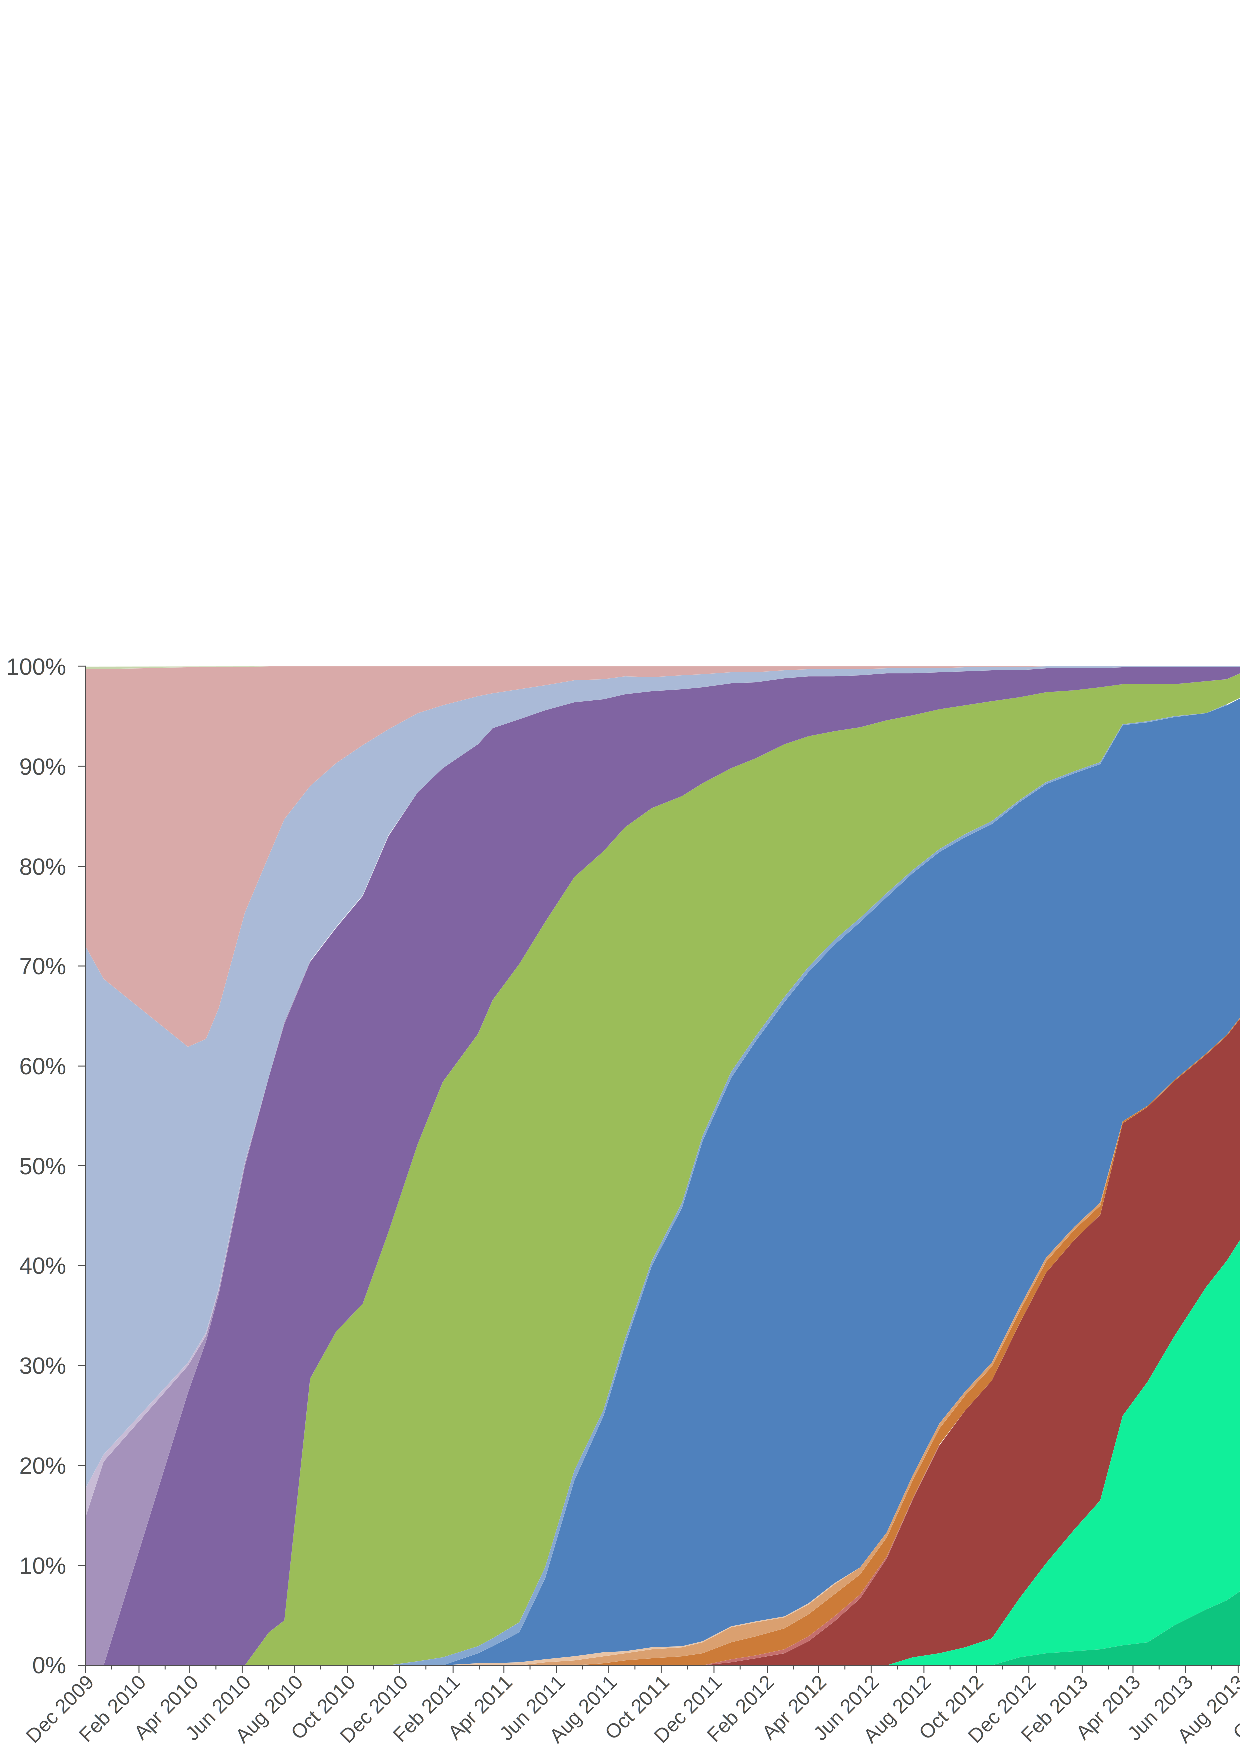
\includegraphics[width=\linewidth]{figures/android-versions.pdf}
% %\caption[Historical Android version's distribution.]{Historical Android
% %  version's distribution~\cite{erikrespo_android_2017}.}
% %\label{fig:android-versions}
% %\end{figure}
% 
% The data devices store is highly personal. Smart watches
% record and shared a user's pulse with others. Mobile health apps track and
% check medical conditions. In the US, the \ac{HIPAA} regulation requires that
% healthcare providers transmit medical information securely, but many apps have
% basic security problems~\cite{fahl_why_2012}, and many of the healthcare apps
% do not handle information securely~\cite{knorr_privacy_2015}.
% 
% Software is predominantly distributed through app stores.
% To install an app on an early mobile device the user would
% download it on a traditional computer and then transfer it to the
% mobile, where they could install it using a package manager.  App
% stores have made this simpler by allowing users to find
% an install apps straight from their device.  Whilst the app store is
% the normal method of installing apps, apps can still be downloaded and
% installed manually by side-loading on Android or through iTunes for
% iOS.
% 
% On Android Google's Play Store is often the
% default app store but users are free to choose other marketplaces if they wish.
% One choice is Amazon's Appstore.  It is the default for Amazon's
% Kindle Fire tablets, and has special offers for Amazon customers.
% Other marketplaces are regional.  In China, where Google web services
% cannot be used, alternative markets such as Qihoo360 and Baidu have
% appeared.

\section{Thesis Outline and Publications}

The rest of this thesis is organised into the following chapters.
Some of the work described has been presented at various conferences, workshops and PhD symposiums through the course of the PhD.
We describe the publications, and show where they fit into the various chapters.

\begin{itemize}
\item \emph{Chapter 2: Background.} 
  Describes Becker~\etal's work on SecPAL, and gives an overview of work developing policy languages.

\item \emph{Chapter 3: Instantiating and Evaluating SecPAL.} 
  Introduces AppPAL as a language instantiating SecPAL to describe the policies
  of the mobile ecosystem. We introduce the language through examples before
  showing how we implemented it. We also describe some modifications to the
  language from SecPAL to make writing policies easier. We conclude by describing
  our tools for analyzing AppPAL policies for satisfiability and redundancy
  errors.
  
  Some of the early examples were taken from our paper:
  \begin{itemize}
  \item\emph{Towards an authorization framework for app security
      checking~\cite{hallett_towards_2014}.} A PhD symposium paper describing how
    we might use SecPAL to model policies in the mobile ecosystem.
  \end{itemize}

\item \emph{Chapter 4: App Stores and App Preferences.} 
  Having described AppPAL, start to describe the differences betweeen different
  app stores and survey their different terms and conditions. We use AppPAL to
  capture descriptions of user's app privacy preferences; and measure the extent
  users follow these preferences when selecting apps by comparing with records of
  user's app installation history. Finally we describe a tool for generating
  \emph{curated} app stores on the basis of a policy.
  
  Some of the implementation described, and work on capturing user's privacy preferences is included in our papers:
  \begin{itemize}
  \item\emph{AppPAL for Android~\cite{hallett_apppal_2016}.} Describes AppPAL as an instantiation of SecPAL.  Presents evaluation algorithm.  Shows how to capture user privacy preferences as AppPAL policies and tries to find examples of users following the policies in a user app-installation dataset.
  \item\emph{Poster: Using Authorization Logic to Capture User Policies in Mobile Ecosystems~\cite{hallett_poster:_2015}.}  Presents early work measuring the extent users seem to follow an AppPAL translation of user privacy prefences.
  \end{itemize}

\item \emph{Chapter 5: Applying AppPAL to BYOD Policies.}
  We move from describing \emph{user-centric} policies, to ones companies might
  want to enforce. We look at how we can capture BYOD policies using AppPAL by
  looking at five BYOD policies (which are given in Appendix A). In capturing the
  policies, we identify two idioms that existing MDM tooling does not capture. We
  also describe how AppPAL could be used to enforce a BYOD policy by integrating
  with existing tooling.
  
  This chapter encompasses and extends our work presented in:
  \begin{itemize}
  \item\emph{Capturing Policies for BYOD~\cite{hallett_capturing_2017}} Describes work on using AppPAL to capture the rules and trust relationships in BYOD policies.
  \item\emph{Common Concerns in BYOD Policies~\cite{hallett_common_2017}.} Describes work looking at BYOD policies to find common areas of concern.  
  \item\emph{Specifying BYOD Policies with Authorization Logic~\cite{hallett_specifying_2016}.} PhD symposium paper describing early work capturing BYOD policies with AppPAL.  Shows how we could use AppPAL to look for common problems, such as completeness.
  \end{itemize}

\item \emph{Chapter 6: Future Work.}
  Describes possible future work, including a probabilistic variant of AppPAL.
 
\item \emph{Chapter 7: Related Work.} 
  Describes XACML and DKAL, to related policy languages. We also give an overview
  of the various \emph{fine-grained permissions systems} for Android that can be
  used to enforce some policies.
\end{itemize}



\end{document}


%%% Local Variables:
%%% mode: latex
%%% TeX-master: "../ch1"
%%% End:
